\documentclass{report}

\usepackage{multirow}
\usepackage[francais]{babel}
\usepackage[latin1]{inputenc}
\usepackage{times}
\usepackage[T1]{fontenc}
\usepackage{amsmath}
\usepackage{graphicx}
\usepackage{listings}

\begin{document}

\chapter{V\'ehicule}
\section{Description du v\'ehicule \label{TableDesc}}
La voiture sur laquelle nous nous basons est un model r\'eduit
t\'el\'ecomand\'e de type 4x4. Le tableau suivant est un inventaire de 
ses caract�ristiques en son \'etat actuel:

\begin{center}
  \begin{tabular}{|p{4cm}|p{4cm}|c|}
    \hline
    \multirow{5}{*}{Grandeurs}
    &longueure & 35 cm \\ \cline{2-3}
    &longueure (centre de roue \`a centre de roue)& 17 cm \\ \cline{2-3}
    &largeure & 22 cm \\ \cline{2-3}
    &largeure (centre de roue \`a centre de roue) & 17 cm \\ \cline{2-3}
    & hauteur au sol & 4 cm\\ \hline
    \multirow{3}{*}{Moteur de propulsion}
    & Voltage de marche & \~{}5V - \~{}10V  \\ \cline{2-3}
    & Courant min (roue libre) & \~{}2A \\ \cline{2-3}
    & Courant max (roue bloqu\'ee) & \~{}3A \\ \hline
    \multirow{5}{*}{Servo de guidage}
    & Fabriquant & Corona \\ \cline{2 - 3}
    & Model & Metal gear DS558HV\\ \cline{2-3}
    & Voltage de marche & \~{}6V - \~{}7.4V  \\ \cline{2-3}
    & Courant & 300mA - 400mA \\ \cline{2-3}
    & Charge maximale & 12kg - 14kg \\  
 \hline
	\end{tabular}
\end{center}

\subsection{System directionel initial}
Dans son \'etat initial, le syst\`eme de guidage pouvait se comparer \`a un
servo tr\`es rudimentaire. Il en comptait toutes les caract�ristiques, mais en
un �tat simplifi�, en particulier le syst�me de positionnement. Dans un servo
classique, il s'agit d'un potentiom�tre (variateur de r�sistance) qui permet
de savoir en tout moment la position de la corne. Par contre, dans le cas de
la voiture, un syst�me de balais (voir image) assure cette t�che. Il en
r�sulte une identification de position tr�s basique: gauche, droit ou
droite.\\
(ins\'erer images)\\
Sachant que nous avons retir\'e l\'electronique de la voiture, il nous restait
deux possibilit\'es: utiliser le syst\`eme de guidage rudimentaire, mais
d\'ej\`a en place ou tout remplacer avec un servo conventionel.\\
Apr\`es beaucoup de temps perdu \`a tenter de contr\^oler le guidage de base
avec notre \'electronique import\'ee, on d\'ecide de passer \`a un servo. On
ach\`ete un puissant servo de haute qualit\'e chez une connaissance qui en
avait command\'e un gros lot pour la modique somme de 10.- CHF.

\subsection{Remplacement du System de guidage}
Une instalation fiable d'un objet \'etranger dans un ensemble usin\'e tel la
voiture n'est pas t\^ache facile. Il fallait pourtant que le r\'esultat final
soit solide, si l'on voulait compter dessus. C'est pour cela que nous avons
cr\'e\'e une base en contreplaqu\'e pour y loger le Servo.

Ce montage permet de retirer le servo en cas de besoin, donc de pouvoir le
remplacer. En effet, la plaque sup\'erieure est fix\'ee au moyen de vices \`a
bois. Le servo est accompagn\'e, dans son logement, d'un morceau de gomme
adh\'erante (morceau de chambre \`a air). La structure \'epouse les formes de
la voiture pour un maximum de rigidit\'e. La transmission de la force aux
roues se fait par l'interm\'ediare d'une tige de m\'etal. Celle-ci, est
fix\'ee \`a la corne du servo et \`a une boucle soud\'ee \`a l'ancien axe de
transmission. Nous utilisons justement l'ancien axe de transmission pour une
raison d\'evelop\'ee plus tard (voir :
http://en.wikipedia.org/wiki/Ackermann\_steering\_geometry sur
``Ackerman steering'').

\subsection{contr\^ole du servo}
Le contr\^ole d'un servo est un devoir qu'un microcontr\^oleur tel que
l'arduino effectue avec aise. On peut indiquer \`a un servo de se rendre vers
un de ses $180^{\circ}$ de libert\'e en lui envoyant un signal \'electrique dit
modul\'e. Ce signal est modul\'e d'une mani\`ere comprh\'ensible pour le
servo. L'illustration suivante
pourrait d'avantage \'eclairer le lecteur:

\begin{figure}[h]
\centering
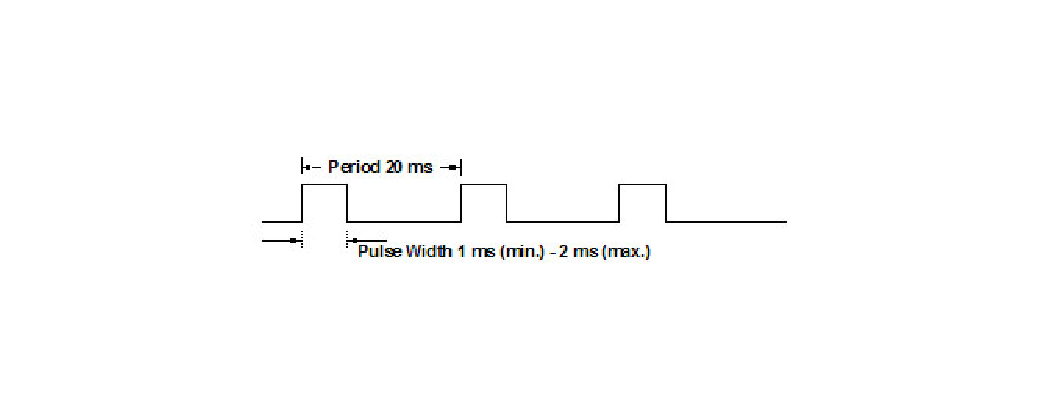
\includegraphics[width=1.0\textwidth]{figures/ServoPwm}
    \caption{\label{ServoPwm}Sch\'ema de la modulation du signal
      \'electrique \protect\footnotemark}
\end{figure}

\footnotetext{Wiki sur les Servos: http://en.wikipedia.org/wiki/File:ServoPwm.png }
Comme l'on peut voir, le dit signal, est form\'e de hauts et de
bas. Lorsqu'il est ``bas'', cela veut dire que la tension est basse ou \'egale
\`a 0V. Lorsqu'il est
``haut'', cela veut dire que la tension est a une valeure d\'efinie auparavant,
standard, diff\'erente de 0V. Dans notre cas, ``haut'' est \`a 5V (standard
pour le mod\'elisme et l'\'electronique en g\'en\'eral). On appelle la
p\'eriode pendant laquelle le signal est ``haut'' une pulsation.

Chaque d\'ebut de pulsation est s\'epar\'e par un temp bien d\'efini de
20ms. Ce qui peut varier d'une pulsation \`a l'autre, donc ce qui informe le
servo en quel angle il doit se positionner, est la longueur de la
pulsation. Comme indiqu\'e, celle-ci peut varier de 1ms \`a 2ms.

\subsection{Programmation pour contr\^oler un servo}
Le programme suivant est un exemple propos\'e dans la section
``apprentissage'' du site officiel d'Arduino. Il utilise la librairie
``Servo'' install\'ee avec l'IDE Arduino. Ce que font les m\'ethodes de cette
classe est de produire un signal comme celui discut\'e \`a la section
pr\'ec\'edente et l'\'emettre par le pin choisi.

Les commentaires sont en anglais, mais le code sera expliqu\'e tout de suite:

\lstinputlisting[language=Java]{code/ServoExample.java}

\textbf{Commentaires:}

On commence par inclure la class Servo, puis on cr\'ee un objet
\emph{Servo}. Dans la partie emph{setup} du programme, on lie l'objet
\emph{myservo} au pin 9 de l'arduino. Ensuite, dans la partie \emph{loop}, on
fait varier la position du servo gr\^ace \`a la m\'ethode \emph{write}. Un
d\'elai(le programme s'arr\^ete en ce point) de 15ms pour permettre au servo
d'atteindre la position demand\'ee. Etant donn\'e que cette op\'eration est
itt\'er\'ee plusieurs fois au moyen d'une boucle \emph{for}, on pourra voir le
servo d\'ecrire un mouvement de balayage.

D'ailleur, ce programme est tr\`es pratique pour tester le fonctionement d'un servo. 

\section{Moteur de propulsion}

\subsection{Descriptif}

Le moteur de propulsion, au contraire du servo, est l'original de la
voiture. Ses caract\'eristiques \'electriques (donn\'ees que nous avon mesur\'e \`a l'aide
d'un multim\`etre du gymnase) se trouvent \`a la section
(\ref{TableDesc}). Le moteur est muni d'une boite \`a vitesse ainsi qu'un
diff\'erentiel. Nous avons estim\'e qu'il aurait \'et\'e
inutilement compliqu\'e d'y apporter quelques modifications qu'ils soient. La
configuration d\'ej\`a existente, \`a l'exception de l'\'electronique,
subvient tout \`a fait \`a nos besoins.  

\subsection{H-bridge}
Faire tourner l'axe d'un moteur \'electrique pose peu de probl\`emes. Il
suffit de connecter l'un des p\^oles \`a la tention positive et l'autre \`a la
n\'egative. Ceci fera tourner l'axe du moteur dans un sens. Si vous souhaitez le
faire tourner dans le sens inverse, il suffit d'\'echanger les fils
\'electriques aux p\^oles du moteur.

Le probl\`eme suivant se pose alors: comment inverser le sens de marche du
moteur sans intervention manuelle?

La r\'eponse est donn\'ee par un astucieux circuit compos\'e de
transistors. Il permet, au moyen de deux signaux actionnant les transistors,
de contr\^oler le sens du courrant passant dans le moteur.

Le sch\'ema suivant pourra d'avantage \'eclairer le lecteur:

\begin{figure}[h]
\centering
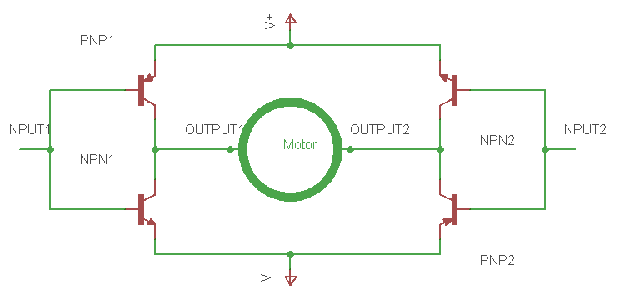
\includegraphics[width=1.0\textwidth]{figures/H-bridge}
    \caption{\label{H-bridge}Sch\'ema d'un H-bridge}
\end{figure}

\textbf{Explications:}

Tout d'abord, que sont des transistors NPN et PNP? La diff\'erence pratique
entre ces deux types de transistors est que l'un demande un signal
d\'eclencheur haut pour \^etre ouvert tandis que l'autre en demande un
bas ou la terre. Dans ce cas, on utilise deux types de transistors
diff\'erents (en grande partie pour clarifier le sch\'ema), mais l'on pourrait
tr\`es bien utiliser uniquement des transistors du m\^eme type. On obtiendrait
le m\^eme r\'esultat en connectant les \emph{INPUT} \`a des transistors
diagonalement oppos\'es.\footnote{Explications inspir\'ees par les informations
trouv\'ees sur le site suivant: http://www.robotroom.com/BipolarHBridge.html}

On peut voir que selon le \emph{INPUT}, on obtiendra des tensions au bornes du
moteur ou \emph{OUTPUT} variables.
\subsection{Table de V\'erit\'e}
R\'edigeons un tableau de v\'erit\'e pour mieux illustrer la situation, o\`u H
(high) signifie haut et L (low) signifie bas :

\begin{table}[h]
\begin{center}
  \begin{tabular}{c|c||c}  
    \emph{INPUT1} & \emph{INPUT2}
    & Tension\\
    \hline
    H & L & \emph{OUTPUT1} $=$ \emph{OUTPUT2}\\
    L & H & \emph{OUTPUT1} $=$ \emph{OUTPUT2}\\
    H & H & \emph{OUTPUT2} $>$ \emph{OUTPUT1}\\
    L & L & \emph{OUTPUT1} $>$ \emph{OUTPUT2}\\
  \end{tabular}
\end{center}

\caption{\label{tableDeVerite} Table de v\'erit\'e accompagnant le sch\'ema du
H-bridge (fig.(\ref{H-bridge}))}

Quand les signaux \emph{INPUT} sont oppos\'es, le moteur est \`a
l'arr\^et. Quand ils sont \'equivalents, le moteur est en marche, dans un sens
ou dans l'autre.

\end{table}

\subsection{Code}

Maintenant que nous avons compris le fonctionement d'un H-bridge, en
particulier les cons\'equences d'\emph{INPUT} diff\'erents, on pourra cr\'eer
un petit programme Arduino pour contr\^oler un moteur.

Le code suivant a \'et\'e r\'edig\'e par Eric:

\lstinputlisting[language=Java]{code/motor.java}

\end{document}
